%% The first command in your LaTeX source must be the \documentclass command.
%%
%% Options:
%% twocolumn : Two column layout.
%% hf: enable header and footer.
\documentclass[
    hf
]{ceurart}
\usepackage[top=2.5cm, bottom=2.5cm, left=2.5cm, right=2.5cm]{geometry}

%%
%% One can fix some overfulls
\sloppy

%%
%% Minted listings support 
%% Need pygment <http://pygments.org/> <http://pypi.python.org/pypi/Pygments>
\usepackage[frozencache,cachedir=./_minted-bdi]{minted}
%% auto break lines
\setminted{breaklines=true}
\usepackage[utf8]{inputenc}	% allow utf-8 input
\usepackage{placeins} % for FloatBarrier
\usepackage{lipsum}
\usepackage{tabularx}
\usepackage{metrix}


%%
%% end of the preamble, start of the body of the document source.
\begin{document}

%%
%% Rights management information.
%% CC-BY is default license.
\copyrightyear{2024}
\copyrightclause{Copyright for this paper by its authors.
    Use permitted under Creative Commons License Attribution 4.0
    International (CC BY 4.0).}

%%
%% This command is for the conference information
% \conference{CHR 2022: Computational Humanities Research Conference, December 12 -- 14,
%     2022, Antwerp, Belgium}
\conference{}
%%
%% The "title" command
\title{Bootstrap Distance Imposters: A less accurate classifier for a more civilized age}

% \tnotemark[1]
% \tnotetext[1]{I would like to thank various members of the Computational
%     Stylistics Group \url{https://computationalstylistics.github.io/} for their
%     ideas and support}

%%
%% The "author" command and its associated commands are used to define
%% the authors and their affiliations.
\author[1]{Ben Nagy}[%
    orcid=0000-0002-5214-7595,
    url=https://github.com/bnagy/bdi-paper,
    email=benjamin.nagy@ijp.pan.pl,
]
\address[1]{Institute of Polish Language, Polish Academy of Sciences (IJP PAN)\\
    Adama Mickiewicz 31\\
    Kraków, Poland}
%%
%% The abstract is a short summary of the work to be presented in the
%% article.
\begin{abstract}
    This paper describes an update to Mike Kestemont and Walter Daeleman's
    open-source Python implementation of the General Imposters method of
    authorship attribution. The new algorithm, called Bootstrap Distance
    Imposters (henceforth BDI), incorporates several of the improvements
    proposed since the code was last updated in 2015, as well as introducing a
    novel method of bootstrapping that has several attractive properties when
    compared to the reference algorithm. The two approaches are benchmarked
    using the problems from the PAN 2014 author identification task
    \cite{pan_2014}, and some additional properties of BDI are showcased via
    real-world case studies. BDI is shown to be a high-precision (few false
    positives) classifier for authorship attribution, with competitive overall
    accuracy, and significant advantages in interpretability.
\end{abstract}

%%
%% Keywords. The author(s) should pick words that accurately describe
%% the work being presented. Separate the keywords with commas.
\begin{keywords}
    authorship attribution \sep
    stylometry \sep
    bootstrapping \sep
\end{keywords}

%%
%% This command processes the author and affiliation and title
%% information and builds the first part of the formatted document.
\maketitle

\section{Introduction}

The General Imposters method (henceforth GI), originally formulated by M. Koppel
and Y. Winter in \cite{koppel_gi}, has become one of the standard
methods for authorship attribution. After strong performances in the PAN 2013 and
2014 competitions, it was implemented and used by M. Kestemont et al. in an
influential study \cite{kestemont_caesar}, improved by N. Potha and E.
Stamatatos in 2017 \cite{potha_improved_gi}, and is now available in the
well-known R package \emph{stylo} \cite{stylo}.

In this paper I describe an update to Kestemont's open-source Python
implementation \cite{kestemont_ruzicka} called Bootstrap Distance Imposters (henceforth BDI) which
incorporates several of the improvements proposed since the last release, as
well as introducing a novel method of bootstrapping that has several attractive
properties when compared to the reference algorithm. The two approaches are
benchmarked using the problems from the PAN 2014 author identification task
\cite{pan_2014}, and some additional properties are showcased via real-world
case studies.

\section{Motivation and Design}

The GI method is, in machine learning terms, an ensemble classifier. These
classifiers regularise well, but while they produce a real-valued output, it is
problematic to interpret this as a probability. The output of the Kestemont GI
classifier is a percentage of binarized `votes' (the number of times a candidate
text was closer than an imposter).

In contrast, the raw output from the BDI algorithm is a bootstrapped
distribution of differences. At each step, the distance (with a bootstrapped
feature set) between the candidates and the imposters is recorded, using any
vector distance measure $d: \mathbb{R}^n \times \mathbb{R}^n \rightarrow
    \mathbb{R}$. If the candidates are further, the difference between the distances
is negative, if closer it is positive. If these individual distances follow a
Gaussian distribution (which is a reasonable prior expectation) then their
difference is also Gaussian. Expressing the results this way has some
advantages. The first is that we can differentiate a negative result (not the
candidate) as either `none of the above' or `more like an imposter' (the true
author is in the imposters set). A `none of the above' result would have a
statistically expected distance of zero (equally unlike the candidate and the
imposters), and so we would see a distribution centred around 0.%
%
\footnote{ Note carefully that this is a one-way implication---a true author
    that is neither the candidate nor one of the imposters should have a
    distance distribution centred around zero, but not all such distributions
    guarantee that the true author is not among the imposters.}
%
On the other hand, `more like an imposter' results show distributions centred
around a negative value (examples of this can be seen in Section
\ref{sec:showcase} below). The other advantage is that for strong positives, we
have additional data about the match. Distributions centred around larger
positive numbers are better matches, but distributions with high variance show
more feature dependence (since the strength of the match varies greatly
depending on the bootstrap features). In summary, positive matches (with most or
all of the probability mass above zero) can be much more meaningfully compared.

It is worth noting here that the overall best performing method at PAN 2014 by
M. Khonji and Y. Iraqi \cite{khonji_iraqi} also modified the classic GI
algorithm to incorporate the distance between vectors (in that case the relative
distance of the test vector to candidates vs imposters is used in the decision
function for a `standard' voting-based classifier), so this paper is not the
first to note the utility of this additional information.

\subsection{Classification Performance}

Based on the BDI algorithm, which outputs a distribution, it is obviously useful
to have a summary statistic that can be interpreted as evidence for authorship
attribution tasks. For this paper I used a simple approach that considers the
amount of probability mass that lies above 0. If every test is closer to a
candidate that an imposter then the result will be 1, if every test is more like
an imposter, it will be 0, etc. This is implemented as
\texttt{(100-scipy.stats.percentileofscore(x, 0)) / 100.0}, the inverse
percentile of (a distance of) 0. Thus armed with a method that outputs a
`probability-like' result in $[0,1]$, I wrapped the code in a classifier that
follows \texttt{sklearn} \cite{scikit-learn} conventions like \texttt{fit()} and
\texttt{predict\_proba()}  and evaluated the BDI classifier directly against the
updated Kestemont GI \texttt{Order2Verifier}, using the 2014 PAN authorship
attribution problems. This provided a convenient benchmark, and also the
opportunity to compare the results against a number of other (although older)
verification approaches.

\subsection{Score Shifting}

The PAN 2014 competition provided a set of training problems, and the c@1 metric
introduced in that competition rewards (or at least penalises less harshly)
classifiers that choose not to answer some problems. This leads naturally to
algorithms that use the training data to define classifier output ranges that
will be assigned to 0.5 (indicating an unanswered problem). In the case of
classic GI, this means that classifier scores (vote percentages) within certain
ranges will be rectified to 0.5, hopefully improving the c@1 score as compared
to basic accuracy.

The score shifting method implemented in Kestemont GI attempts to produce
something more like a probability by linearly scaling the output values. The
code defines an upper and lower bound for the unanswered region, \texttt{p1} and
\texttt{p2} The scaling code (in Python) looks like this:

\begin{minted}{python}
    for score in list(scores):
        if score <= p1:
            new_scores.append(rescale(score, min(scores), max(scores), 0.0, p1))
        elif score >= p2:
            new_scores.append(rescale(score, min(scores), max(scores), p2, 1.0))
        else:
            new_scores.append(0.5)
\end{minted}

Scores below \texttt{p1} are scaled to $[0,\texttt{p1})$, scores above
                \texttt{p2} are scaled to $(\texttt{p1},1]$, and the rest are coerced to 0.5.
There is an issue with this scaling algorithm, however. Since \texttt{p1} and
\texttt{p2} are chosen by grid search to maximise the PAN score, the score
shifter sometimes fits values for \texttt{p2} that are well below 0.5. This can
lead to decisions that are defined as positive (since they are above
\texttt{p2}) being scaled to below 0.5, where they are evaluated by the scoring
metrics as a negative result (and scored as such). In the updated code I
modified the shifting code to scale more simply to $[0,0.5)$ (negative), 0.5
                (unanswered), and $(0.5,1]$ (positive). This does not retain the global
distributional properties of the original results (as in Kestemont).

\begin{minted}{python}
    for score in scores: 
        if score <= p1: 
            new_scores.append( rescale(score, orig_min=0, orig_max=p1, new_min=0.0, new_max=0.499) ) 
        elif score >= p2: 
            new_scores.append( rescale(score, orig_min=p2, orig_max=1, new_min=0.501, new_max=1.0) )
        else: 
            new_scores.append(0.5)
\end{minted}

Based on the evaluation problems, the BDI algorithm is not as sensitive to this
score shifting, deriving only a modest benefit from fitting. The fitting process
raises natural questions about the representativeness of the training data, and
also causes some problems in domains that suffer from limited data availability
(where it can be hard to sacrifice data for training). In these circumstances, BDI
works well with manual score shifting, allowing the user to choose a confidence
level based on first principles.

\subsection{Changes to Kestemont GI}

As is the nature of computing, the code in the repository documenting the GI
algorithm and for the related work on the Caesarian corpus no longer ran. I
reworked the code slightly, and made the following small changes, which are
available in my own repository \cite{nagy_ruzicka}.

\begin{itemize}
    \item Update the code to work with Python 3 (these minimal changes have been
          incorporated into the original repository based on a PR)
    \item Implement a fast `nini' metric (fuzzy Jaccard similarity) as described in \cite{nini_aa}
    \item Implement the Potha \& Stamatatos `ranking'
          improvement for the consensus score%
          %
          \footnote{ Instead of a strict 1 (candidate closest) or 0 (candidate
              not closest), Potha \& Stamatatos proposed a score improvement
              based on the ordinal rank of the closest candidate, so if a
              candidate was the second-closest, the score for that iteration
              would be $\frac{1}{2}$. The same paper proposed a distance-based
              culling method to select more relevant imposters, but this was not
              implemented (with enough bootstrapping this should converge)}
          %
          described in \cite{potha_improved_gi}
    \item Remove most non-core code
    \item Modify the score-shifting algorithm, as described above
\end{itemize}

\subsection{Testing}

\begin{table}
    \caption{Global micro-average results}
    \label{tab:micro}
    % \par\medskip
    \raggedright
    \begin{tabular}{lllcccc}
        \toprule
                                   &               &         & Accuracy       & AUC             & C@1            & Final Score    \\
        Classifier                 & Vectorizer    & Shifter &                &                 &                &                \\
        \midrule
        BDI, Cosine                & 2,3,4,5-grams & fitted  & 0.681          & 0.727           & 0.694          & 0.505          \\
                                   &               & manual  & 0.672          & 0.715           & 0.649          & 0.464          \\
                                   & 2,3,4-grams   & fitted  & 0.686          & 0.723           & 0.689          & 0.499          \\
                                   &               & manual  & 0.681          & 0.715           & 0.645          & 0.461          \\
        BDI, Minmax                & 2,3,4,5-grams & fitted  & \textbf{0.689} & 0.731           & 0.695          & 0.508          \\
                                   &               & manual  & 0.682          & 0.726           & 0.660          & 0.479          \\
                                   & 2,3,4-grams   & fitted  & 0.682          & 0.730           & 0.694          & 0.507          \\
                                   &               & manual  & 0.685          & 0.723           & 0.652          & 0.472          \\
        Kestemont GI, Cosine       & 2,3,4,5-grams & fitted  & 0.673          & 0.768           & 0.695          & 0.534          \\
                                   &               & manual  & 0.621          & 0.698           & 0.557          & 0.389          \\
                                   & 2,3,4-grams   & fitted  & 0.665          & 0.755           & 0.678          & 0.512          \\
                                   &               & manual  & 0.614          & 0.685           & 0.537          & 0.367          \\
        Kestemont GI, Minmax       & 2,3,4,5-grams & fitted  & 0.661          & \textbf{ 0.773} & \textbf{0.702} & \textbf{0.543} \\
                                   &               & manual  & 0.633          & 0.706           & 0.568          & 0.401          \\
                                   & 2,3,4-grams   & fitted  & 0.668          & 0.759           & 0.694          & 0.527          \\
                                   &               & manual  & 0.629          & 0.707           & 0.572          & 0.405          \\
        PAN 2014 Best (individual) &               &         & NA             & 0.718           & 0.684          & 0.490          \\
        \bottomrule
    \end{tabular}
\end{table}

\begin{table}
    \caption{BDI 2,3,4,5-grams, Minmax, Manual Shifter}
    \label{tab:bdi}
    % \par\medskip
    \raggedright
    \begin{tabular}{@{}lrrccccccc}
        \toprule
        Corpus       & Tests & ?? & High Conf. & FP & Acc  . & AUC   & C@1   & Final          & PAN Best       \\
        \midrule
        du\_essays   & 96    & 19 & 75         & 2  & 0.854  & 0.955 & 0.923 & \textbf{0.882} & 0.823          \\
        du\_reviews  & 50    & 10 & 35         & 0  & 0.580  & 0.693 & 0.576 & 0.399          & \textbf{0.525} \\
        en\_essays   & 200   & 27 & 162        & 0  & 0.605  & 0.624 & 0.568 & 0.354          & \textbf{0.513} \\
        en\_novels   & 200   & 34 & 161        & 0  & 0.595  & 0.622 & 0.556 & 0.346          & \textbf{0.508} \\
        gr\_articles & 100   & 34 & 61         & 2  & 0.800  & 0.848 & 0.697 & 0.591          & \textbf{0.720} \\
        sp\_articles & 100   & 35 & 53         & 1  & 0.780  & 0.882 & 0.810 & \textbf{0.715} & 0.698          \\
        \bottomrule
    \end{tabular}
\end{table}

\begin{table}
    \caption{Kestemont 2,3,4,5-grams, Minmax, Fitted Shifter}
    \label{tab:o2v}
    % \par\medskip
    \raggedright
    \begin{tabular}{lrrccccccc}
        \toprule
        Corpus       & Tests & ?? & High Conf. & FP & Acc  . & AUC   & C@1   & Final          & PAN Best       \\
        \midrule
        du\_essays   & 96    & 16 & 54         & 2  & 0.854  & 0.964 & 0.948 & \textbf{0.914} & 0.823          \\
        du\_reviews  & 50    & 12 & 14         & 7  & 0.640  & 0.696 & 0.645 & 0.449          & \textbf{0.525} \\
        en\_essays   & 200   & 14 & 22         & 73 & 0.565  & 0.569 & 0.578 & 0.329          & \textbf{0.513} \\
        en\_novels   & 200   & 42 & 79         & 12 & 0.610  & 0.670 & 0.629 & 0.421          & \textbf{0.508} \\
        gr\_articles & 100   & 28 & 18         & 3  & 0.790  & 0.840 & 0.755 & 0.634          & \textbf{0.720} \\
        sp\_articles & 100   & 15 & 27         & 6  & 0.750  & 0.935 & 0.863 & \textbf{0.807} & 0.698          \\
        \bottomrule
    \end{tabular}
\end{table}

\begin{figure*}
    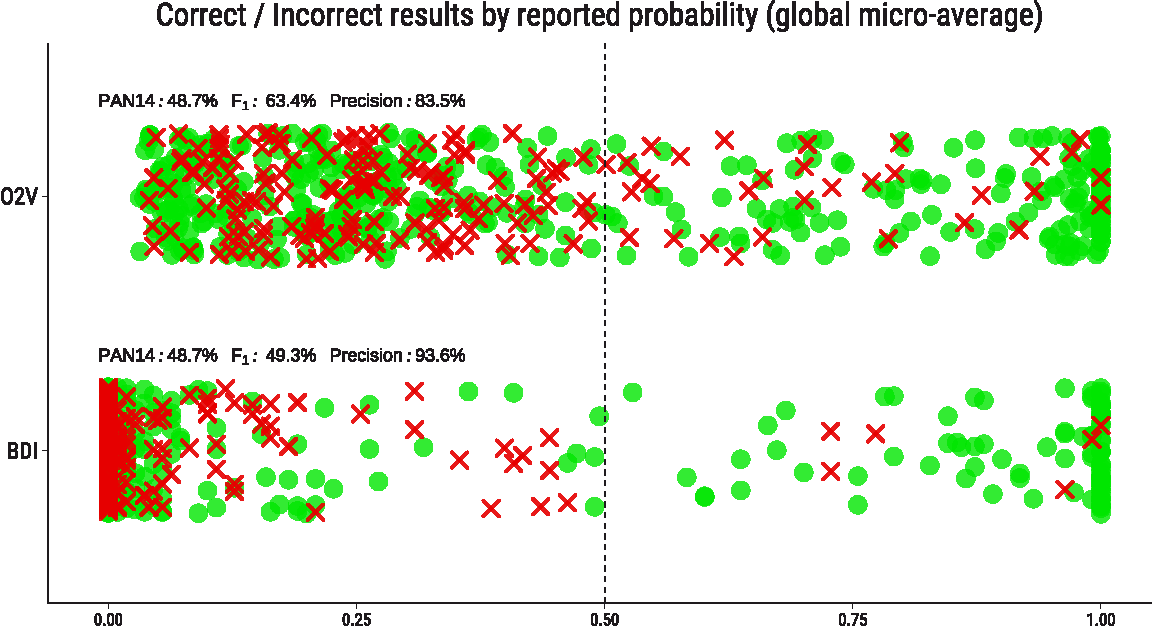
\includegraphics[width=\linewidth]{figures/bdi_o2v-crop.pdf}
    \caption{A comparison of the correct and incorrect results by reported
        probability for BDI (manual shifter, 2,3,4,5-grams, minmax) vs
        Order2Verifer (fitted shifter, 2,3,4,5-grams, minmax)}
    \label{fig:bdi_o2v}
\end{figure*}


The BDI classifier was compared head-to-head with the updated Kestemont
\texttt{Order2Verifier} on the full PAN 2014 evaluation corpus.%
%
\footnote{ There is a small inconsistency that I was unable to resolve---the
    only copy of the verification problems I could find were archived in the
    Kestemont repository, but they are apparently missing 50 of the `Dutch
    Reviews' evaluation problems, so there are a total of 746, versus 796
    reported in the PAN 2014 wrapup report. }
%
For this test I used two different sets of character $n$-grams, since that
feature universe is a generally reliable and uncontroversial choice for modern
authorship attribution work. There may be feature universes that perform better,
or features that work better for a specific task, but character $n$-grams are
`solid if boring'. Likewise, the $n$-gram frequencies are $z$-scaled (based on
the training variances) since this is the `standard' approach. I tested two
$n$-gram configurations, 2,3,4-grams and 2,3,4,5-grams, with fitted and manual
score shifting. Finally, for the distance metric used to determine `closeness'
at each step I tested the cosine distance (the most traditional choice) and the
minmax (Ružička) metric promoted by Kestemont in his original paper. Consistent
with those results, the minmax metric appears generally superior (see Table
\ref{tab:micro}). The fully reproducible testing code is available in the
supplementary repository \cite{nagy_bdi_2024}.

\subsection{Interpretation}

As can be seen from Table \ref{tab:micro}, the performance of the BDI classifier
is consistently strong, with only a small boost in PAN score resulting from
fitting the score shifter. The GI \texttt{Order2Verifier} with a fitted shifter
performs better according to the PAN metrics (deriving a large c@1 benefit from
fitting the score shifter). The GI classifier also appears to outperform the
best overall PAN 2014 entrant by a significant margin. The strength of the BDI
classifiers, however, is twofold: first, they do not really require any training
corpus, and second, the BDI approach is high precision (it yields very few false
positives), making it a conservative classifier whose positive results are
reliable (at the cost of more false negatives). This can be seen clearly in
Figure \ref{fig:bdi_o2v} in which the best performing GI classifier is compared
to the manually fitted BDI classifier (results between 11\% and 89\% are left
unanswered), using the same features and metrics. The results for each subcorpus
are broken down in more detail in Tables \ref{tab:bdi} \& \ref{tab:o2v}.

\section{Showcase}\label{sec:showcase}

In this section I refer to two attribution studies I have contributed to that
are, at the time of writing, still in press. These figures are not full
summaries of the research, but simply illustrate some of the features of the BDI
method that I believe to be useful. As mentioned above, the output of the BDI
algorithm is a distribution of distances, not a summary statistic. These
examples attempt to show that examining the full distribution conveys extra
information and can improve our intuition and confidence in the analysis.

\begin{figure*}
    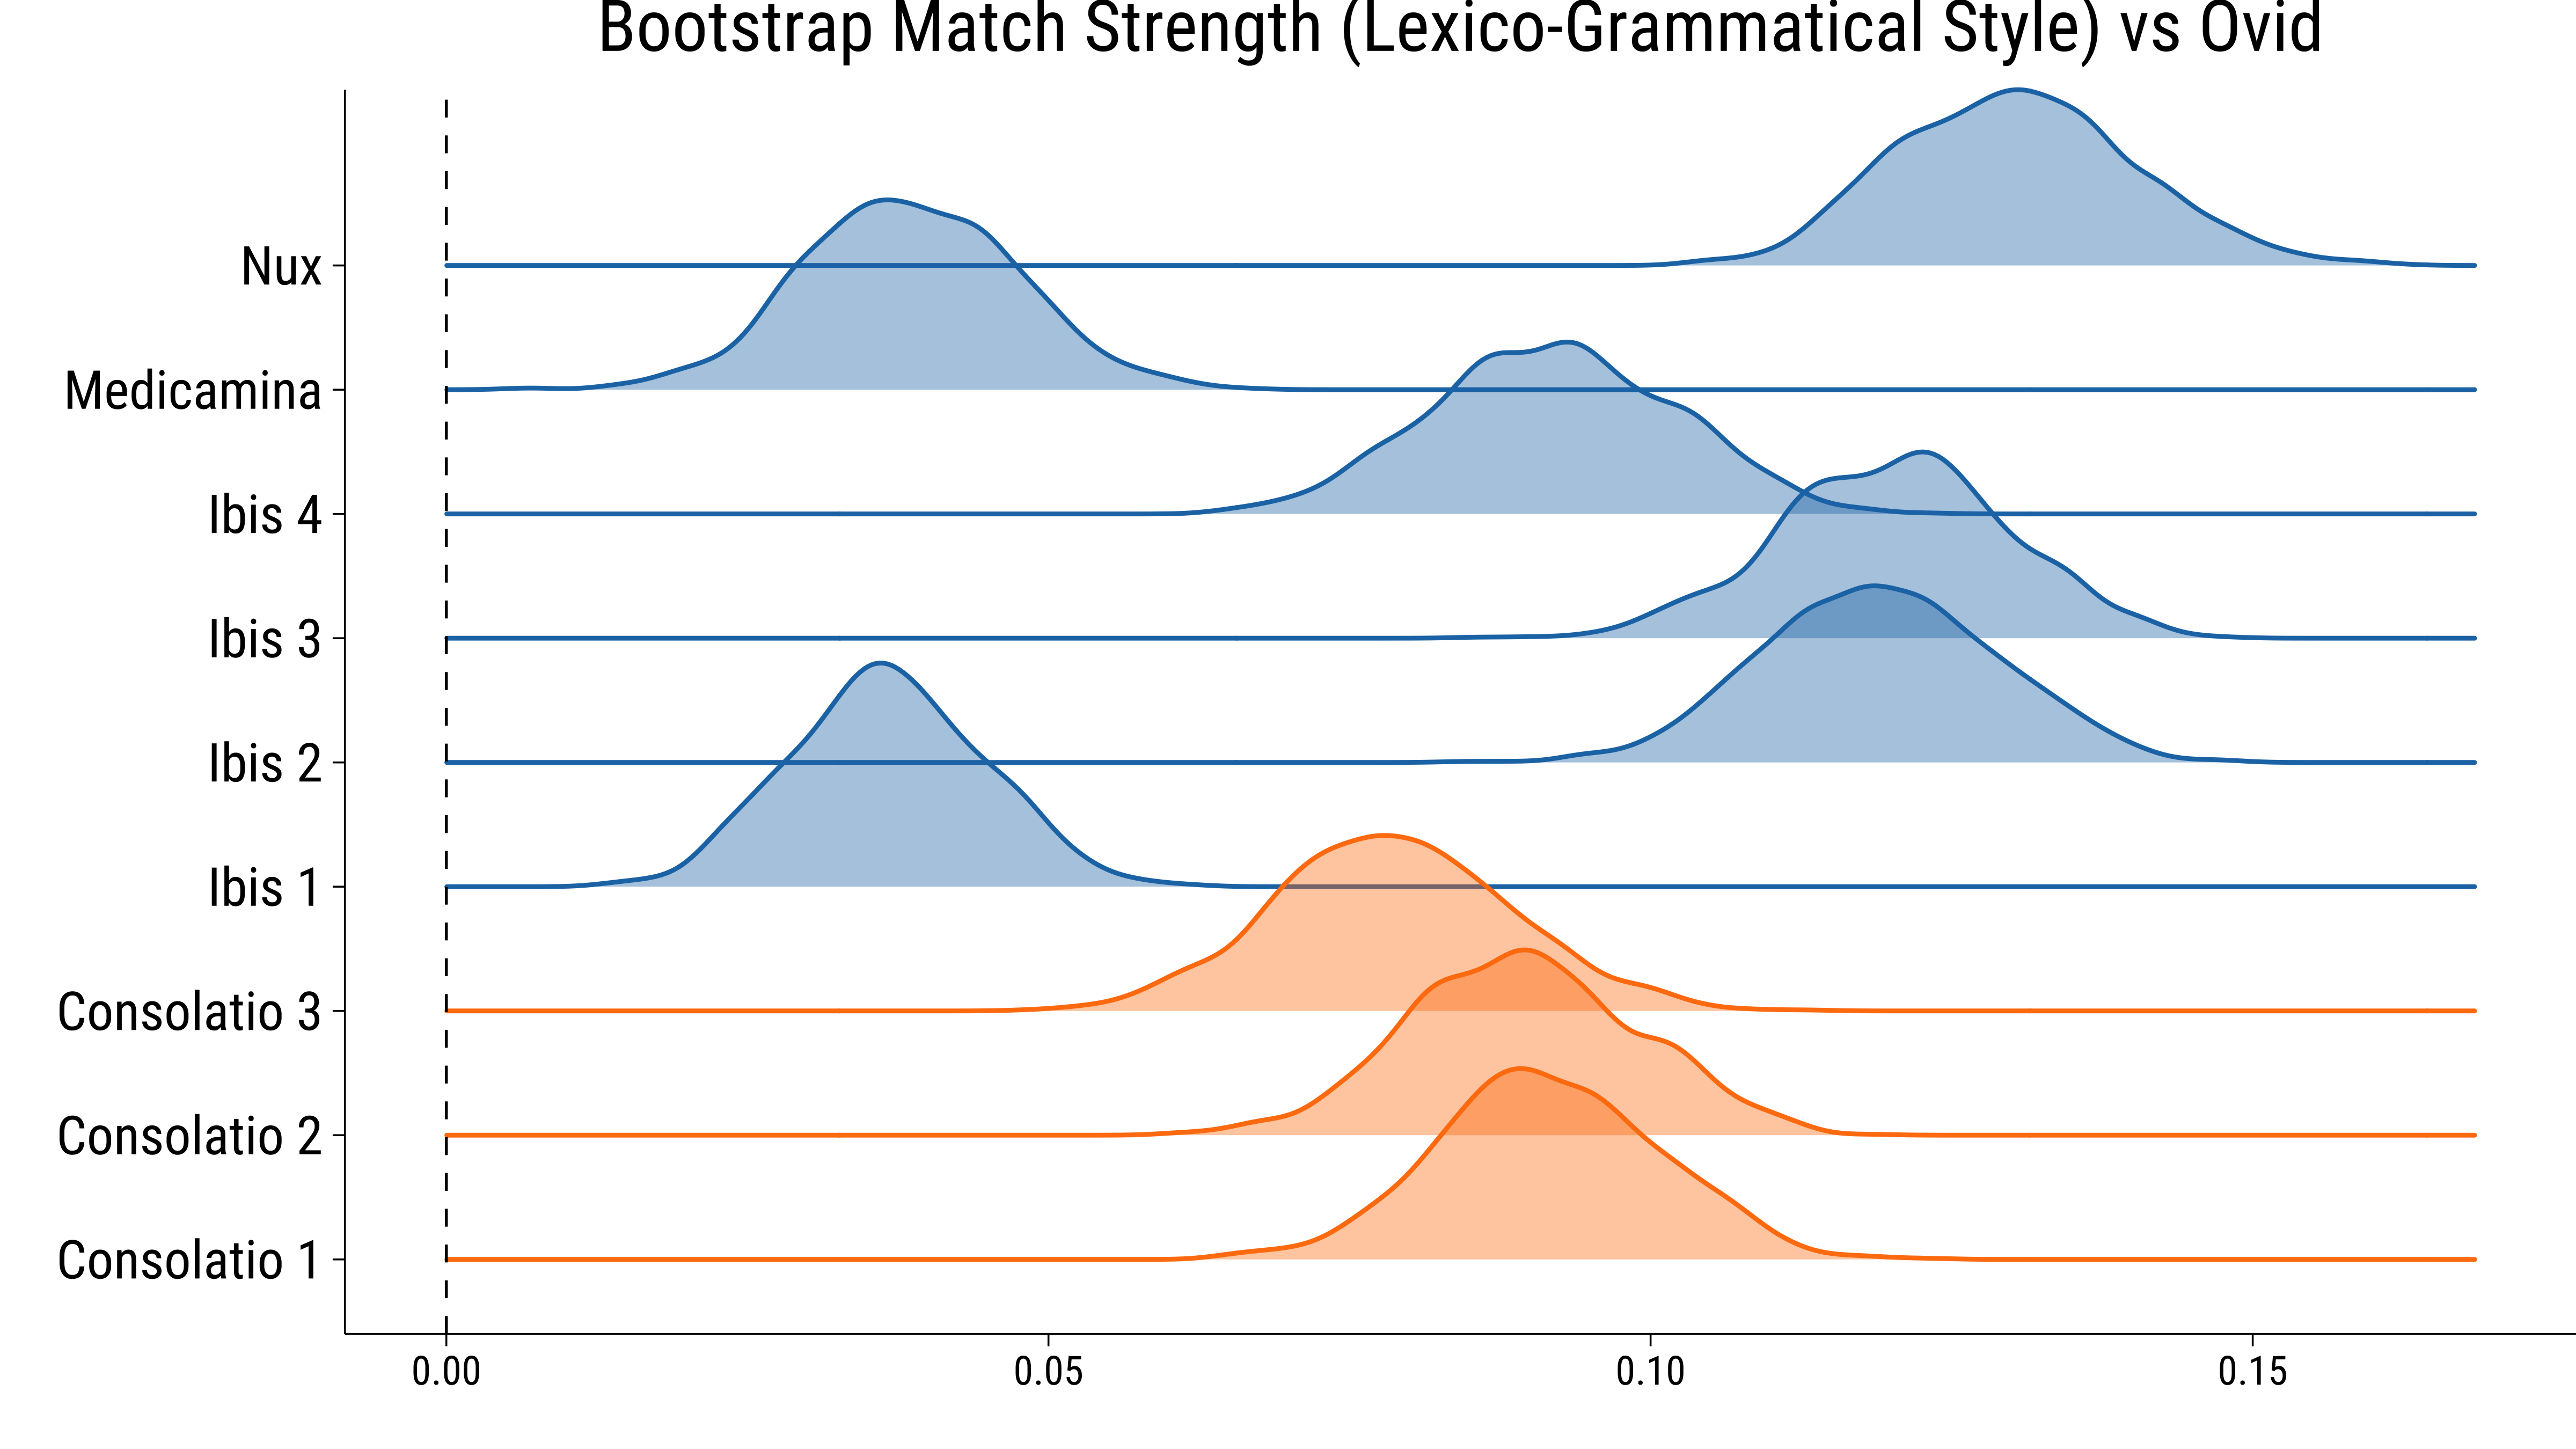
\includegraphics[width=\linewidth]{figures/bootstrap_lexical_paper.png}
    \caption{A BDI comparison of several works attributed to Ovid using
        lexico-grammatical features (character $n$-grams). The \emph{Consolatio Ad
            Liviam} is now considered to be a first-century interpolation.}
    \label{fig:nux_lex}
\end{figure*}

\begin{figure*}
    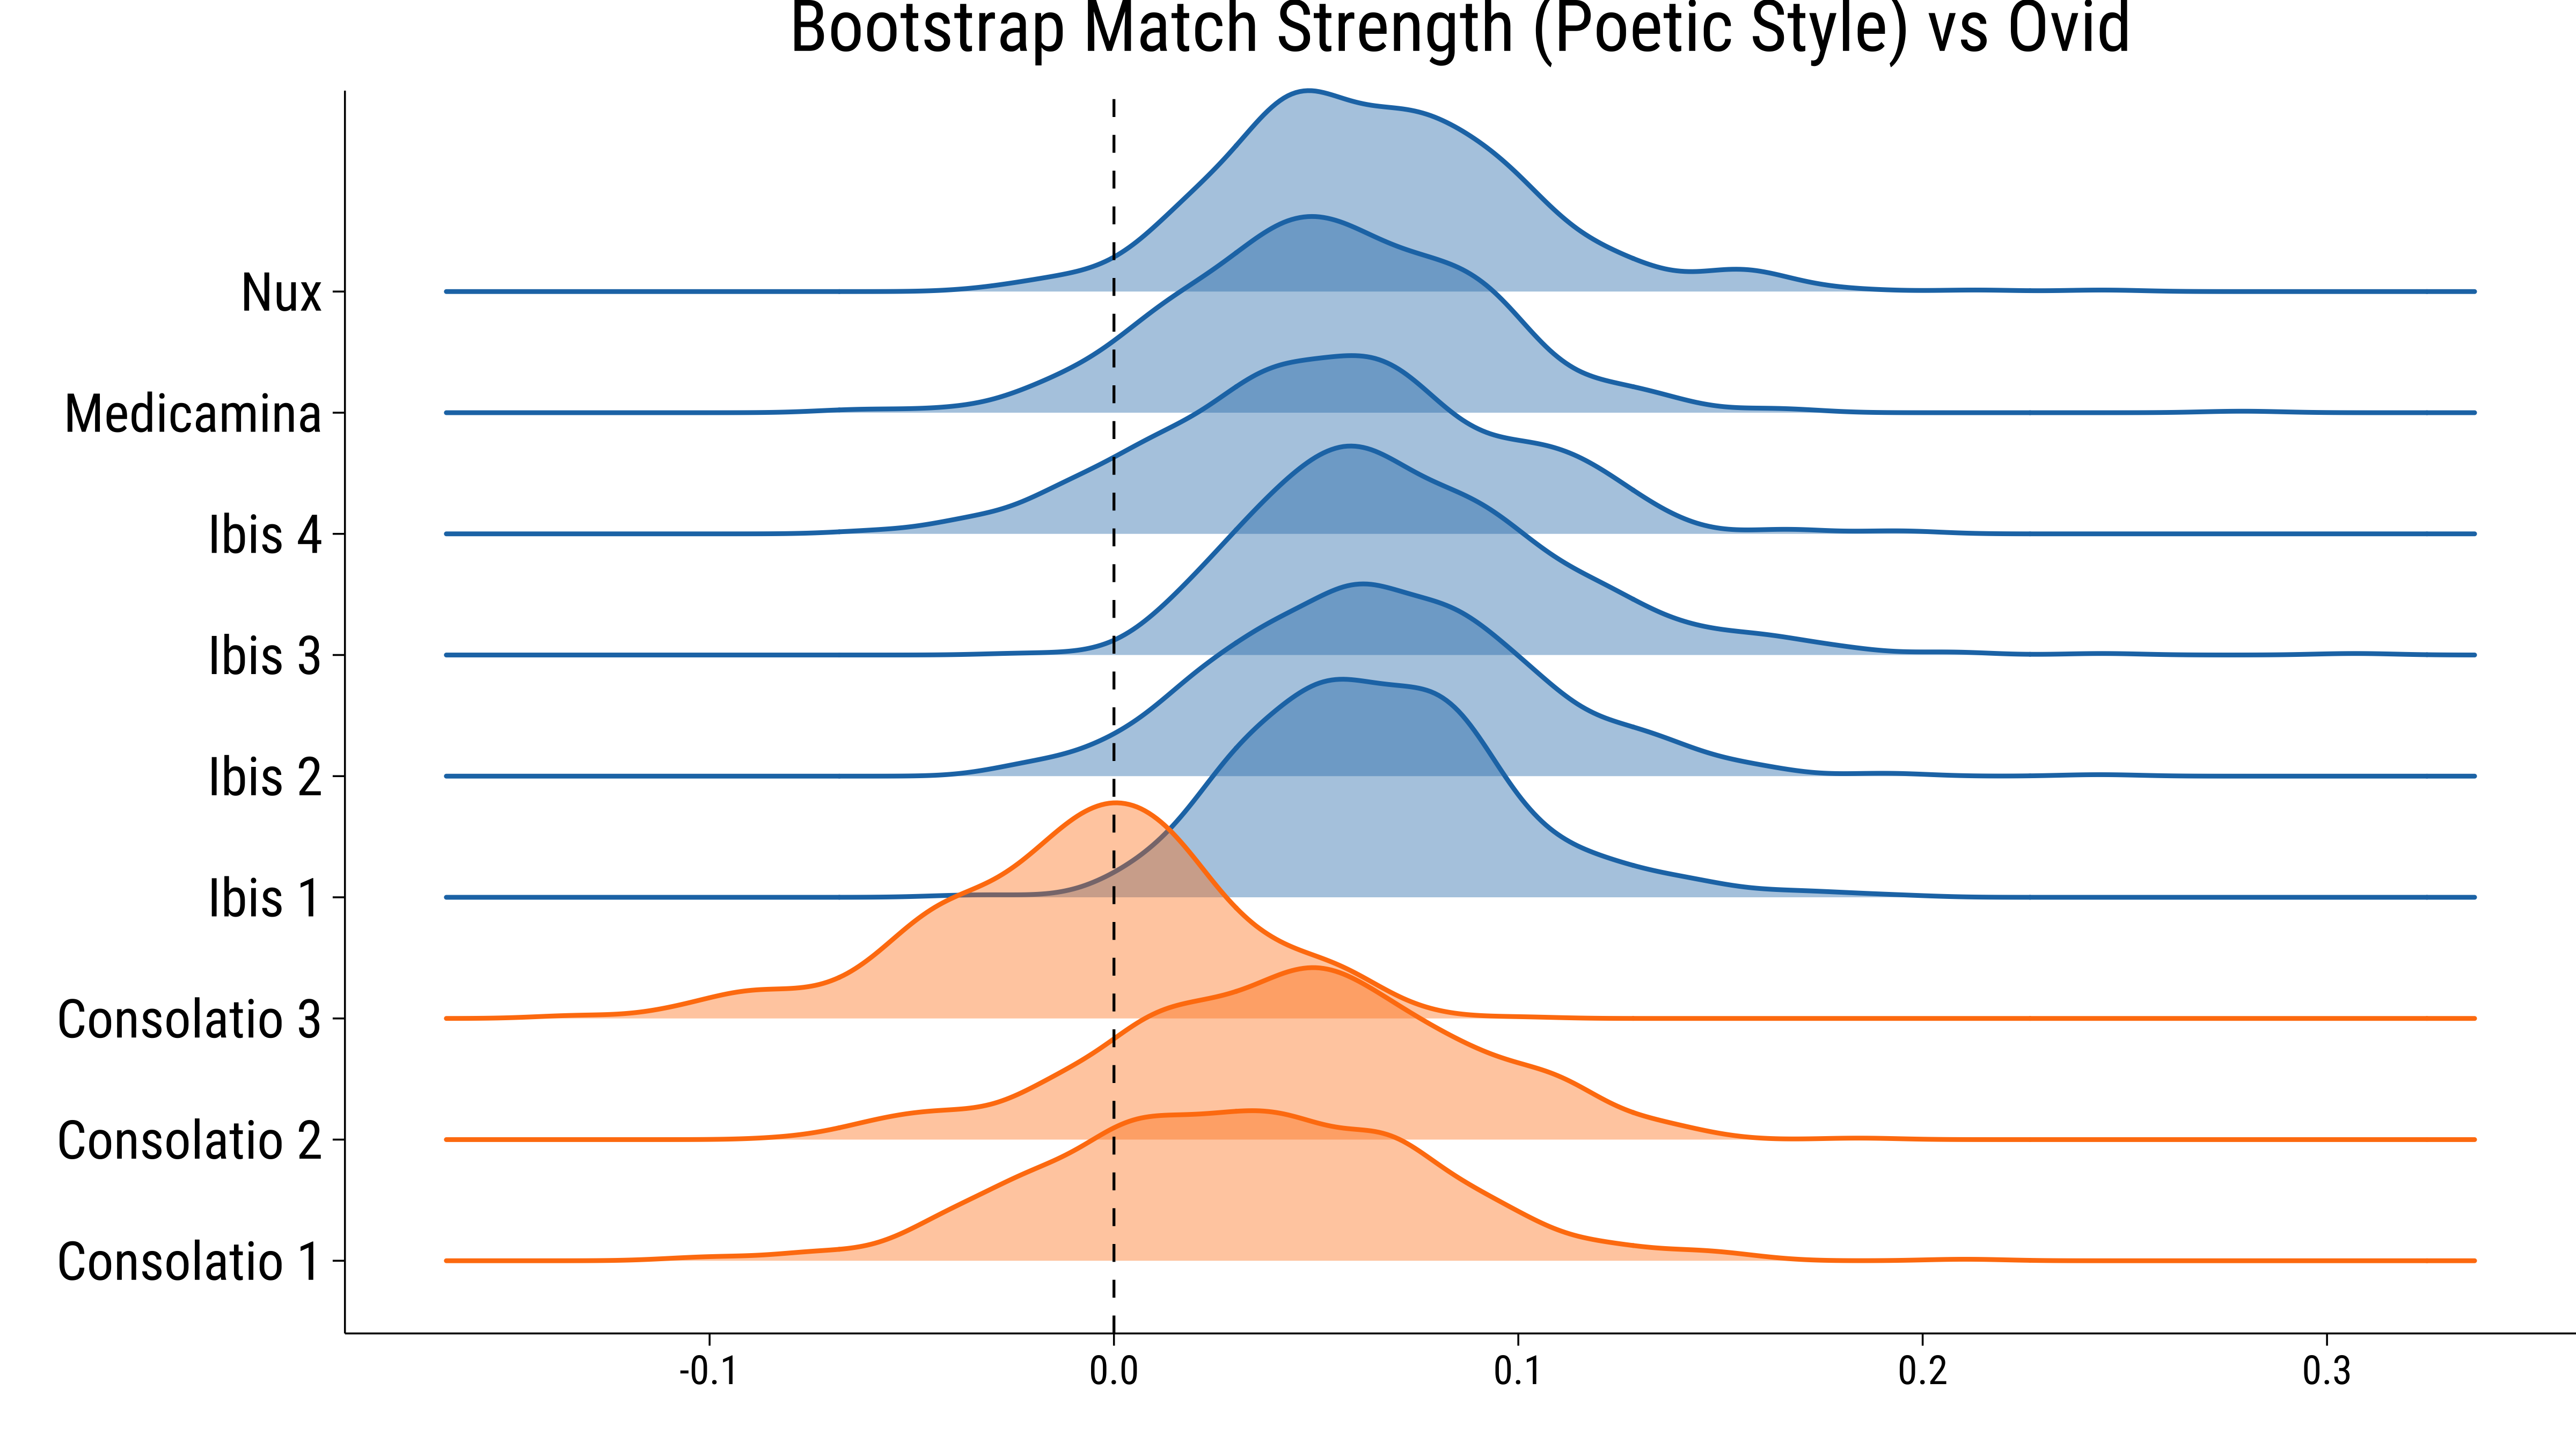
\includegraphics[width=\linewidth]{figures/bootstrap_poetics_paper.png}
    \caption{A BDI comparison of the same works attributed to Ovid, examining
        poetic/metrical features of Latin dactylic elegy instead of lexical
        features.}
    \label{fig:nux_poet}
\end{figure*}

Figures \ref{fig:nux_lex} \& \ref{fig:nux_poet} are from an analysis of several
poems attributed to Ovid. The aim here was to provide evidence for the
genuineness of the \emph{Nux}, but of more interest in this context is the
analysis of the \emph{Consolatio ad Liviam}. The \emph{Consolatio} was once
considered to be a genuine work of Ovid, but is now accepted by most scholars to
be a first-century imitation. By using BDI we attempted to show that metrical
technique was a powerful enough stylistic feature to disambiguate even
deliberate imitation from genuine works. In Figure \ref{fig:nux_lex}, we see the
value of visualising distributions where all of the distances are positive
(closer to the candidate author than an imposter), which would be summarised as
a `probability' of 1.0. This figure measures similarity in terms of
lexico-grammatical features, operationalized as character $n$-grams. In fact, as
can be seen, although the chunks from the \emph{Consolatio} are much more like
Ovid than they are like any of the distractor poets, they are \emph{not as much
    like} Ovid as most of the comparison works. This kind of comparability between
strong matches is very difficult with the standard GI approach. However, in
Figure \ref{fig:nux_poet} which measures metrical features, the difference is
clear---the sections from the \emph{Consolatio} are centered around 0 (or near
enough) as compared to the other works where at least 90\% of the distribution
mass is above 0, representing a positive attribution. This result suggests that
the \emph{Consolatio} is not Ovidian, but also that it is not a good stylistic
match for any of the distractor poets (Tibullus, Propertius, and Catullus).

\begin{figure*}
    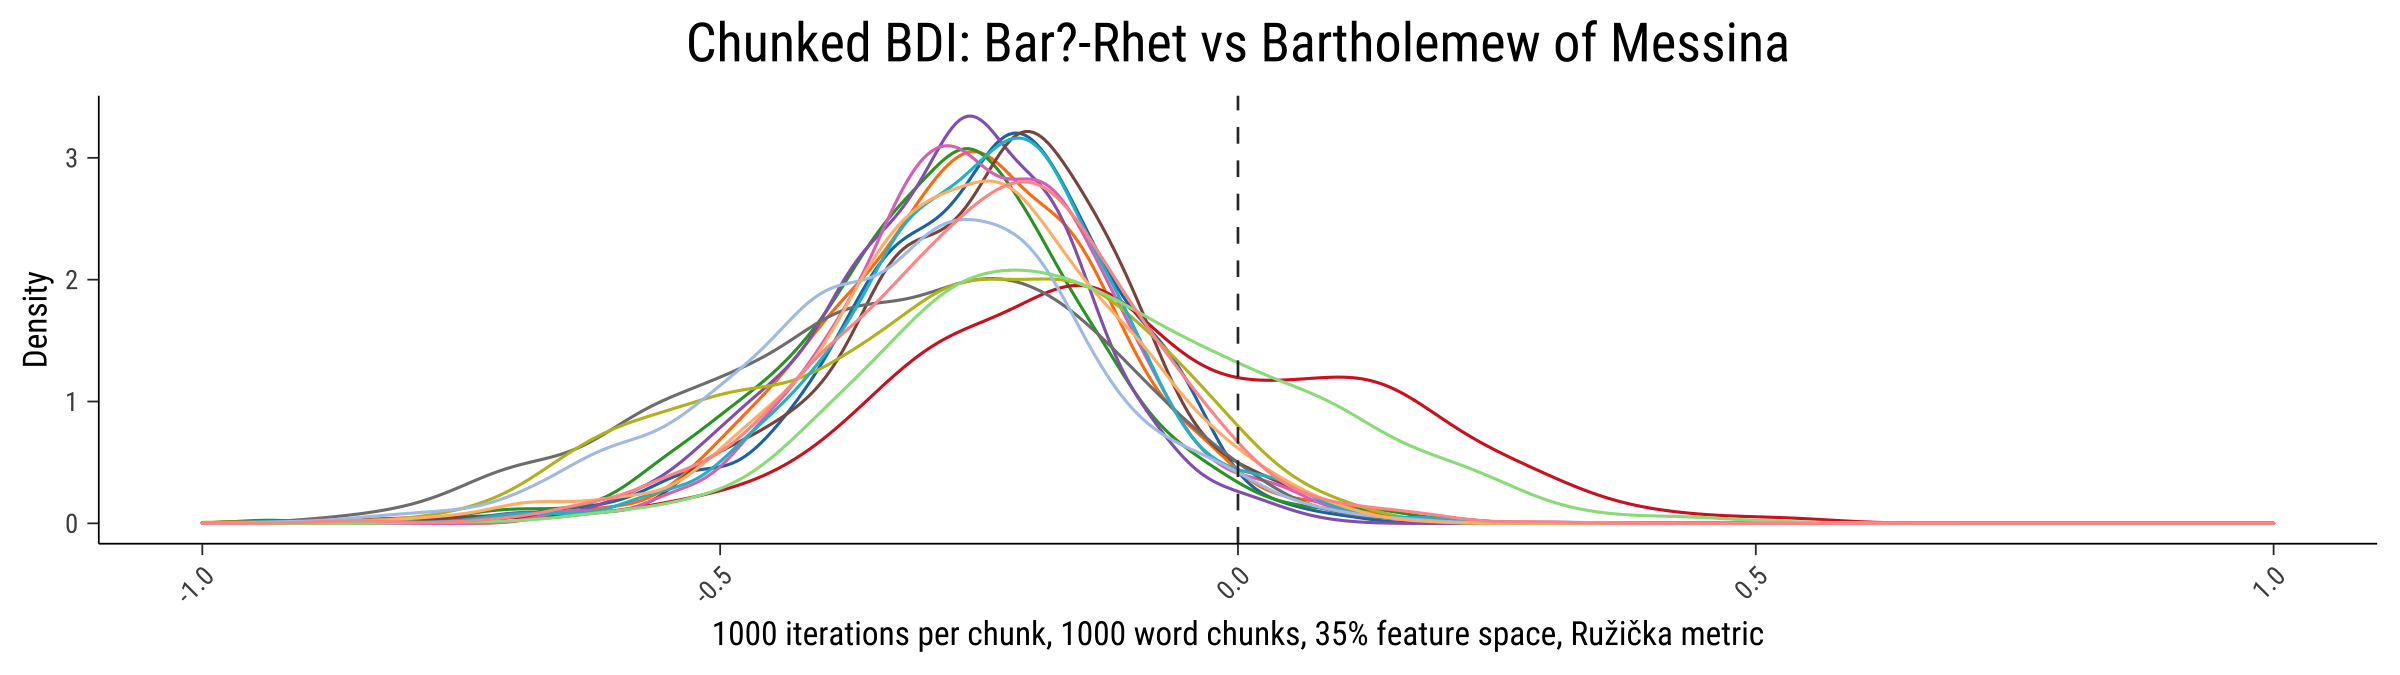
\includegraphics[width=\linewidth]{figures/bdi_bar_paper.png}
    \caption{A BDI comparison of use of Latin function words to match a
        translation of Aristotle's \emph{Rhetorics} to Bartholemew of Messina. Each
        distribution is the full BDI run for one chunk of the work.}
    \label{fig:trans_bar}
\end{figure*}

\begin{figure*}
    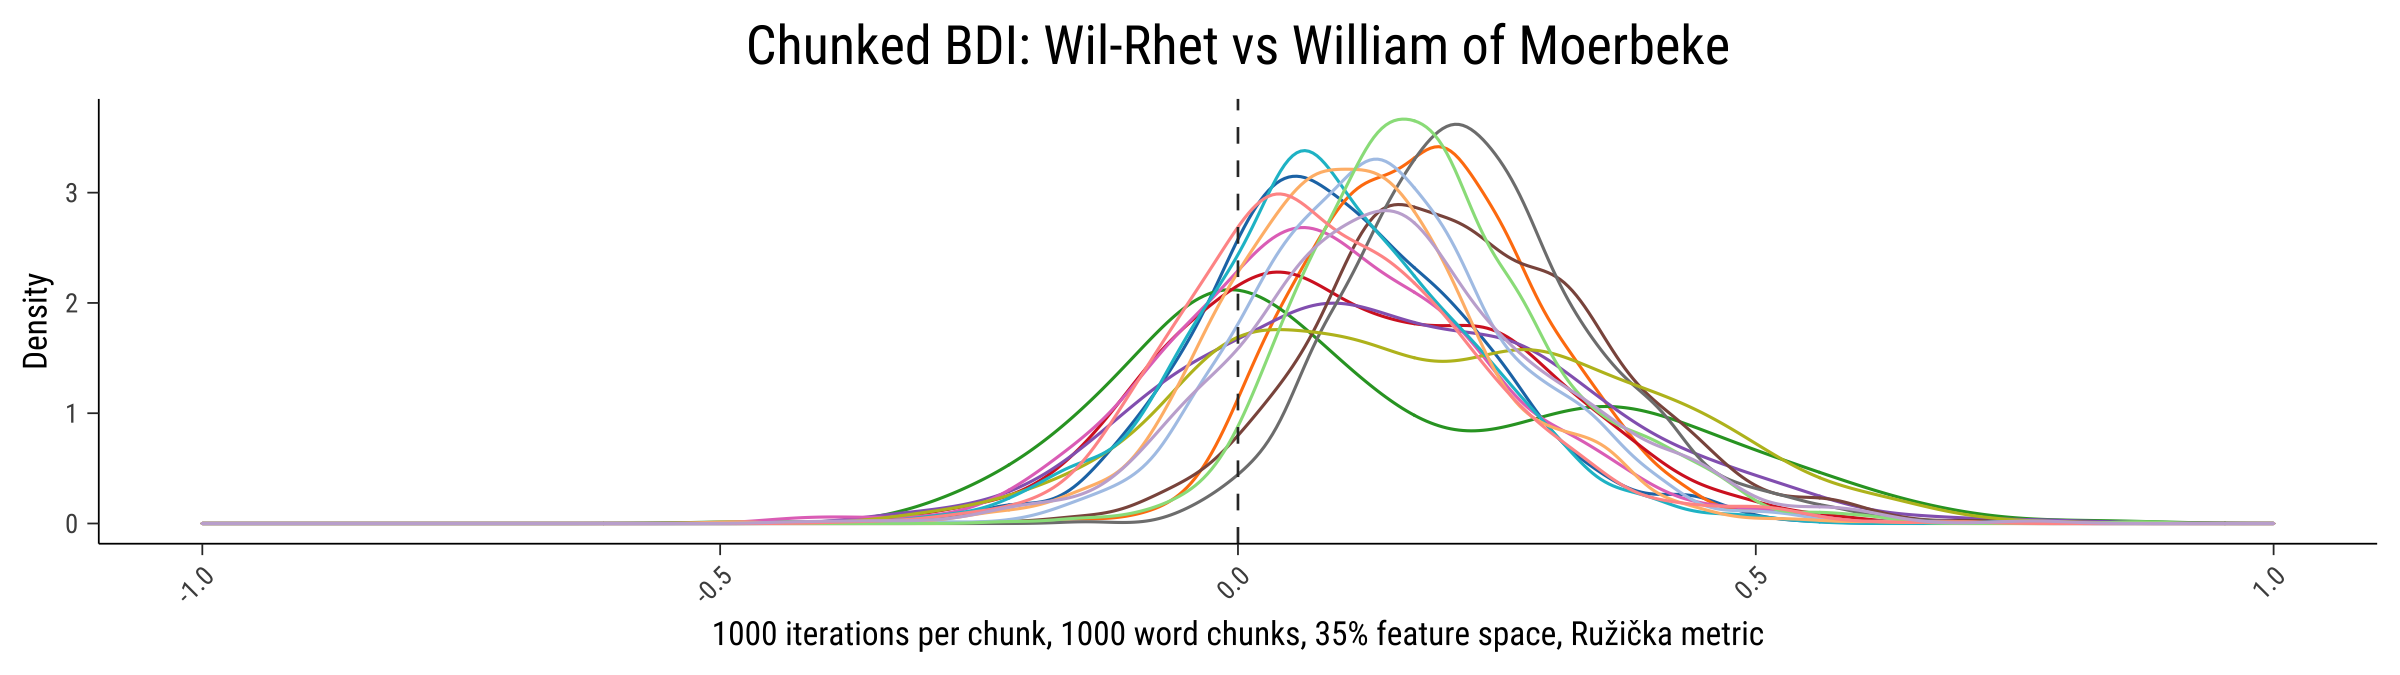
\includegraphics[width=\linewidth]{figures/bdi_wil_paper.png}
    \caption{A BDI comparison of use of Latin function words to match a
        translation of Aristotle's \emph{Rhetorics} to William of Moerbeke. Each
        distribution is the full BDI run for one chunk of the work.}
    \label{fig:trans_wil}
\end{figure*}

Figures \ref{fig:trans_bar} \& \ref{fig:trans_wil} are from an analysis of
translator style, examining medieval translations from Greek to Latin. In this
study, a small set of function words was used, in accordance with the well-known
theory that closed-class words are used more unconsciously, and thus are more
indicative of individual preferences than nouns, verbs, and adjectives which are
highly affected by genre and topic. Overall, this was found to be an effective
approach. Here, however, I note two more useful properties of the BDI method.
The first is that by splitting the work into smaller chunks, and visualising the
distribution for each chunk we are able to see the degree of stylistic variation
in a single translator. It is also clear from Figure \ref{fig:trans_bar} that
some passages are less `stylistically clear', showing much more pronounced
spread---this can be interpreted as greater sensitivity to the individual
feature subsets. Overall, Figure \ref{fig:trans_bar} is centred around a
negative value, indicating that it is significantly more similar to one of the
imposter translators than to Bartholemew. In Figure \ref{fig:trans_wil}, we
performed the same process for a different text that is a translation of the
same work (Aristotle's \emph{Rhetorics}) generally accepted to be by William of
Moerbeke. In this case we see the expected result---almost all of the chunks are
fairly strongly centred around a positive value. The strength of the match is
not as clear as in the Ovidian figures, but this is perhaps to be expected,
since the amount of style that a translator brings to a work can be reasonably
assumed to be less than that brought by an author.

\section{Future Work}

As can be seen from Figure \ref{fig:bdi_o2v}, predictions from the BDI
classifier (after shifting) cluster strongly at the extremes, with most
mis-predictions being high-confidence false negatives. The Kestemont GI
classifier shows the most mis-predictions in the central band (near 0.5), which
is intuitive if the outputs are interpreted as probabilities. The link function
from the BDI distributions to a `probability' in $[0,1]$ is a fairly simple
idea, and can almost certainly be improved to produce a smoother and more
believable distribution across the output range (perhaps logistic regression, or
even empirical distributional statistics). This is left for future work.

\section{Conclusions}

The most common task in authorship attribution work is to positively attribute
works to authors. In this context, although balanced accuracy is not
unimportant, precision (fewer false positives) is often more important than
recall. The c@1 metric introduced for the PAN 2014 authorship verification
competition balances overall AUC (false positives and false negatives) with the
ability for a classifier to decline to answer problems when the result is
unclear. In general, this is a useful innovation, particularly in comparison to
standard machine-learning classifiers which are obliged to assign each problem
to a discrete class (even if the true author is not one of the available
answers). While the GI method performs extremely well, it seems wasteful to
discard the detailed distance information that is calculated in any case during
the bootstrap / voting process.

BDI attempts to address these issues by outputting a full distance distribution
which can be manually inspected. As demonstrated in Section \ref{sec:showcase},
this can be very useful when comparing results that are all strong matches. When
operating as a summary classifier, BDI tends to be conservative in its positive
attributions, showing a false positive rate on the PAN 2014 test problems of
less than 1\% when operating with a score shifter that demanded an 89\%
confidence match. While the raw c@1 results of the BDI
vectorizer/classifier/shifter combinations were not as strong as the best result
from updated Kestemont GI, the fitted versions all outperformed the best PAN
2014 entry, and the more conservative versions (with manual shifting) would all
have finished in the top three. Overall, the BDI approach seems to be a strong
choice, especially where training data is limited and/or reliable positive
results are more important than balanced AUC $\times$ c@1 performance.

\section{Availability of Data and Code}\label{sec:data}

The preprint may be found at \url{https://github.com/bnagy/bdi-paper}. All code
and data is available under CC-BY, except where restricted by upstream licenses.
The code repository includes full reproduction data and code for the evaluation,
as well as various supplemental figures and explanations.

\FloatBarrier

%%
%% The acknowledgments section is defined using the "acknowledgments" environment
%% (and NOT an unnumbered section). This ensures the proper
%% identification of the section in the article metadata, and the
%% consistent spelling of the heading.
\begin{acknowledgments}
    This work was supported by Polish Academy of Sciences Grant
    2020/39 / O / HS2 / 02931.
\end{acknowledgments}

%%
%% Define the bibliography file to be used
\bibliography{bdi_refs}

%%
%% If your work has an appendix, this is the place to put it.
\appendix
\onecolumn

\end{document}

%%
%% End of file